\documentclass{article}

\usepackage{graphicx}

\usepackage[utf8]{inputenc}
\usepackage[T1]{fontenc}
\usepackage[danish,english]{babel}

\usepackage{footnote}
\usepackage{listings}
\usepackage{lastpage}
\usepackage{fancyhdr}

\usepackage{amssymb}
\usepackage{amsthm}
\usepackage{amsmath}
\usepackage{latexsym}
\usepackage{enumerate}
\usepackage{subfigure}

\usepackage[T1]{fontenc}
\usepackage{lmodern}
\usepackage{vaucanson-g}
\usepackage{multido}

\newtheoremstyle{dotless}{}{}{\itshape}{}{\bfseries}{}{ }{}
\newtheoremstyle{itless}{}{}{}{}{\bfseries}{}{ }{}

\theoremstyle{dotless}

\newcounter{maj}
\newcounter{min}

\renewcommand{\thesection}{}
\newcommand{\Section}[1]{\section{#1}
\setcounter{min}{1}}

\renewcommand{\thesubsection}{}

\pagestyle{fancy}
\lhead{Machine Learning, A-1}
\rhead{Kristina Aluzaite (ljg630) and Morten Winther Olsson, hkv518}
\cfoot{\thepage\ of \pageref{LastPage}}

\title{\begin{tabular}{c}
Statistical Methods\\
for\\
Machine Learning\\
Assignment 3\\
\end{tabular}}
\date{18. March 2014}
%% \date{\today}
\author{\begin{tabular}{c}
Kristina Aluzaite (ljg630)\\
Morten Winther Olsson (hkv518)\\
\end{tabular}}

\begin{document}

%% \markboth{Im So Meta Even This Acronym}{Reelect your Teddy Bear}

\maketitle
\thispagestyle{fancy}

\newpage{}

%% \tableofcontents{}

%% \newpage{}

\Section{Introduction}

\Section{III.1 Neural Networks}

\subsection{III.1.1 Neural network implementation}

Code is done, see ``src/Neuron.py''. The random data is generated by \texttt{samples = map(lambda x: (x, (math.sin(x)/x)+np.random.normal(0, .004, 1)[0]), (np.random.rand(1000)*32).tolist())} which should yield data similar to the provided \texttt{sinc} data. Results are in ``Neuron\_stdout''. The backpropagation-wise and numerically calculated gradient differ by more than the assignment text says it should, but still very little. We presume the larger error is due to using floats of limited bit-length in the program.\\

As for the derivative:\\

$h(a)=\frac{a}{1+\vline a\vline}=a\cdot(1+\vline a\vline)^{-1}$\\

Using the product and chain rule gives the derivative.\\

For the case of $a\leq 0$:\\

$h(a)=a\cdot(1-a)^{-1}$\\

and:\\

$h'(a)=(1-a)^{-1}-\frac{a}{(1-a)^2}\cdot -1=\frac{1-a}{(1-a)^2}+\frac{a}{(1-a)^2}=\frac{1}{(1-a)^2}$\\

and since $a\leq 0$, $-a=\vline a\vline$ so $h'(a)=\frac{1}{(1+\vline a\vline)^2}$\\

For the case of $a\geq 0$:\\

$h(a)=a\cdot(1+a)^{-1}$\\

and:\\

$h'(a)=(1+a)^{-1}-\frac{a}{(1+a)^2}\cdot 1=\frac{1+a}{(1+a)^2}-\frac{a}{(1+a)^2}=\frac{1}{(1+a)^2}$\\

and since $a\geq 0$, $a=\vline a\vline$ so $h'(a)=\frac{1}{(1+\vline a\vline)^2}$\\

The derivative includes the case $a=0$ in both cases, and therefore holds continuously across that point.

\subsection{III.1.2 Neural network training}

See ``Neuron\_stdout''. We need to stop gradient descent before overfitting (weights growing to extremes). For small learning rates, it is hard to tell if any progress is made at all, in terms of lowering the error, since the change is so small. However, it is possible to acurately approach the ``ideal'' compromise between low error and least overfitting, while for larger learning rates, the network might be overfitted without warning during a single application. In our case it seems the best learning rate lies somewhere between 0.01 and 1.0. We chose (on gut instinct, (mostly) ignoring validation data outputs) 15 iterations with a 0.1 learning rate for the 2 neuron network, and 30 iterations with a 0.01 learning rate for the 20 neuron network.\\

Plots:\\

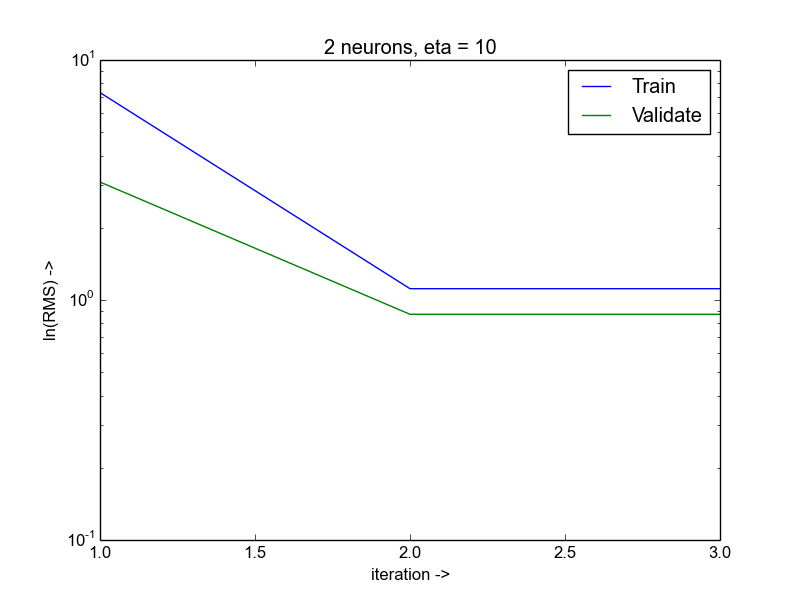
\includegraphics[keepaspectratio=true, width=350pt]{src/img/n_2_eta_10.png}

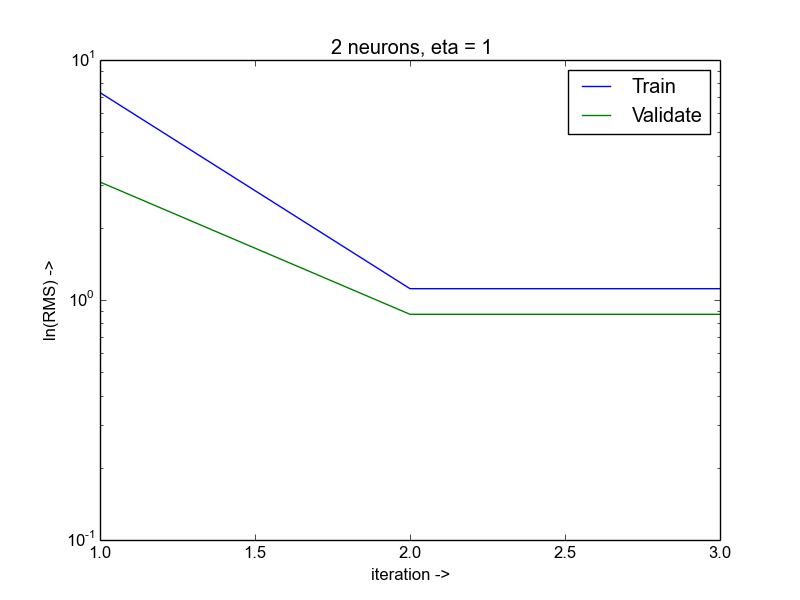
\includegraphics[keepaspectratio=true, width=350pt]{src/img/n_2_eta_1.png}

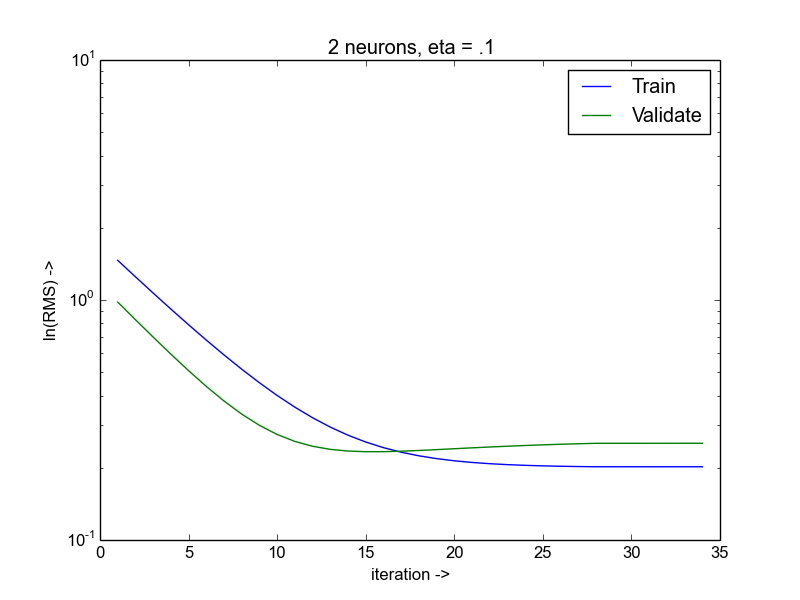
\includegraphics[keepaspectratio=true, width=350pt]{src/img/n_2_eta_01.png}

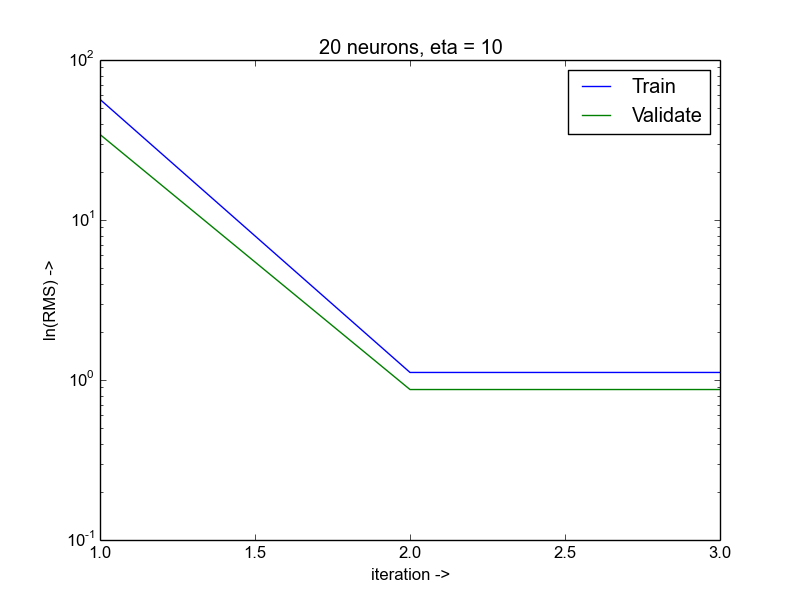
\includegraphics[keepaspectratio=true, width=350pt]{src/img/n_20_eta_10.png}

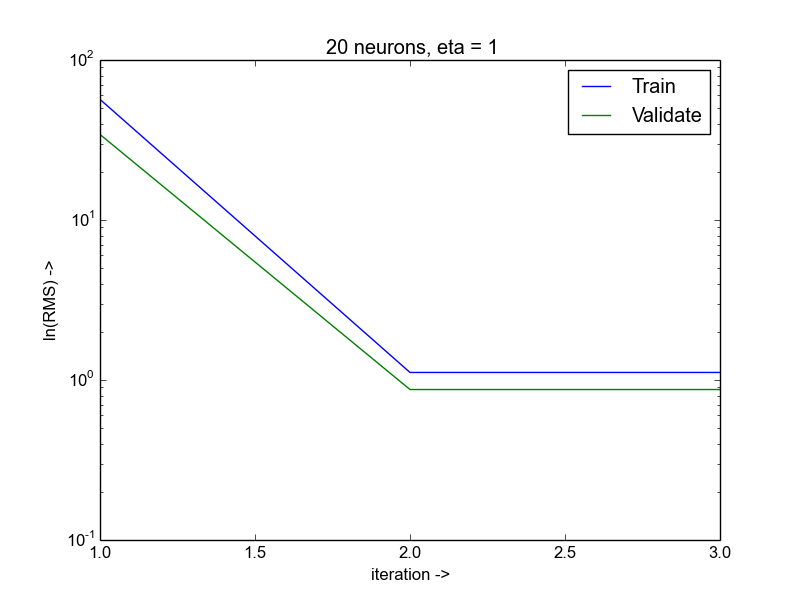
\includegraphics[keepaspectratio=true, width=350pt]{src/img/n_20_eta_1.png}

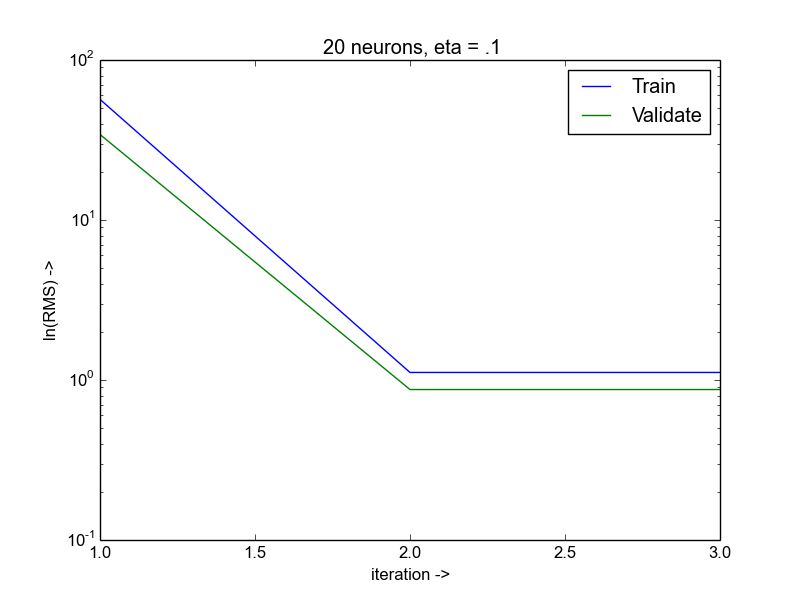
\includegraphics[keepaspectratio=true, width=350pt]{src/img/n_20_eta_01.png}

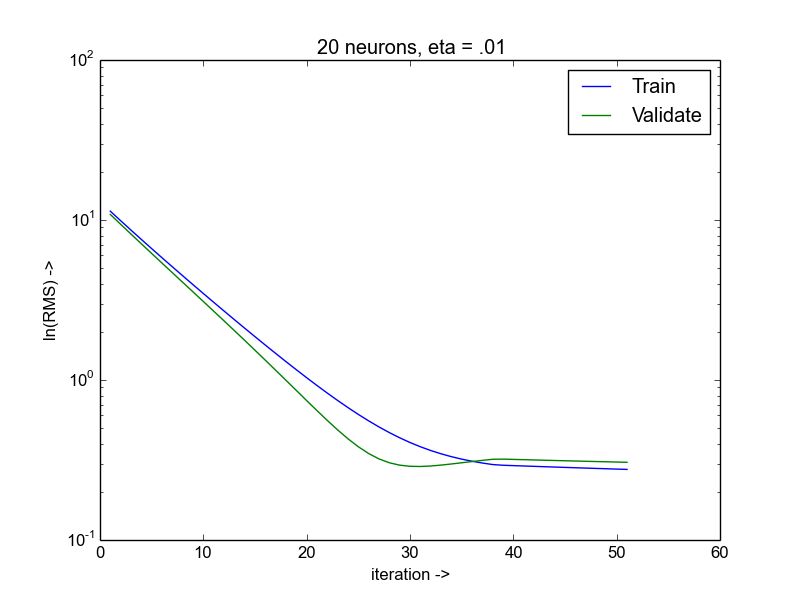
\includegraphics[keepaspectratio=true, width=350pt]{src/img/n_20_eta_001.png}

Plot of combined test of the trained networks\footnote{Yeah, I know the predictions are about as close to the ``right'' values as american right-wing christian fundamentalists, but I'm too tired to care any more, I need sleep :) ... Zzz...}:\\

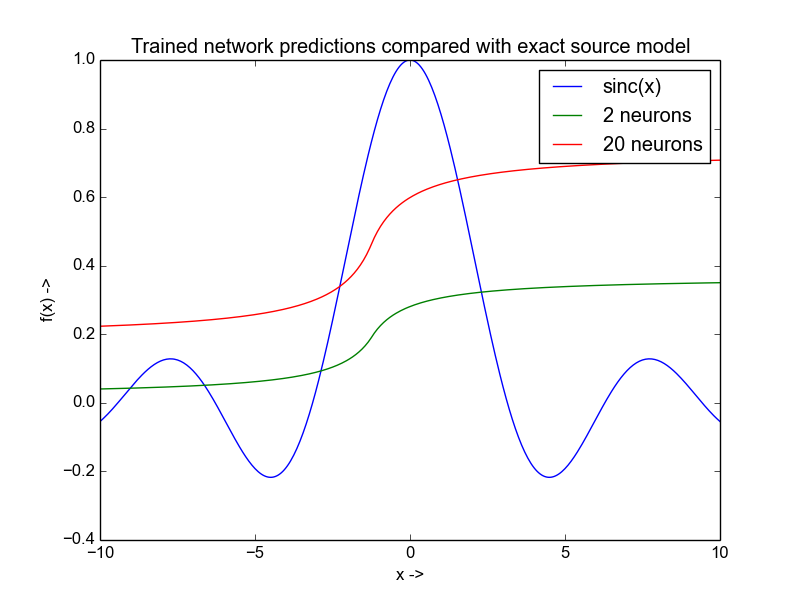
\includegraphics[keepaspectratio=true, width=350pt]{src/img/nn.png}


\Section{III.2 Support Vector Machines}

Done, see ``src/svm\_prob.py''.

\subsection{III.2.1 Data normalization}

Done, see the end of ``SVM\_stdout''.

\subsection{III.2.2 Model selection using grid-search}

Done, see ``src/svm\_prob.py'' and ``SVM\_stdout''. We used the libSVM as advertized in the assignment document. For cross-validation, we defined a higher-order function ``\texttt{partition}'', which, given the number of desired \texttt{folds}, return a function that, given a list, returns a list of \texttt{folds} tuples of two lists made from the original list, where the first member of each tuple contain members whose index modulo \texttt{folds} is not the index of the tuples place in the overall list, and the second tuple member is a list of the remaining members left out from the first list.\footnote{Just look at the code, please, it's not THAT complex, just hard to explain :) ...}\\

It is important to perform numeric input normalization when using SVMs. It places the values of attributes on the same scale, avoiding the bias that would result from attributes of large original scales.  In addition, it makes the data more separable,  resulting in more accurate classification and less error.  The effects of normalization get more pronounced in higher degree polynomial functions.\\

For the raw data we found the best hyper parameters were $C=100$, $\gamma=0.0001$, for normalized data $C=10$, $\gamma=0.1$. The SVM built on raw data predicted the test classification correctly in just over 80pct of the cases, while normalization increased that figure to just over 90pct, as can be seen in ``\texttt{SVM\_stdout}''.

\subsection{III.2.3 Inspecting the kernel expansion}

\subsubsection{III.2.3.1 Support vectors}

During training, \texttt{libSVM} automatically outputs the number of free and bounded support vectors as ``\texttt{nSV}'' and ``\texttt{nBSV}'' respectively. For the final normalized SVM, nSV=56 and nBSV=1, as can be seen in ``\texttt{SVM\_stdout}''. Lower values of C generally yield more bounded SVs but the same amount of free SVs. C is an upper bound on the Lagrange multipliers, and bounded support vectors are those whose multiplier reaches that bound, while support vectors in general are all those that have a Lagrange multiplier $a\geq 0$. If a support vector is not bounded, then it lies on the margin. Thus, if there are no bounded SVs, the data is perfectly separated with a hard margin, which might suggest over-fitting. Lowering C reduces model complexity, and allows more (potentially mis-classified) vectors on the ``wrong side'' of the margin.

\subsubsection{III.2.3.2 Scaling behavior}

If different features of the data are on different scale, numerically larger ones will carry more weight in the separation process. For large data sets, this ``advantage'' can accumulate, meaning that the SVM model will tend to favor the larger feature, to the point of ignoring all others in the infinite limit\footnote{I think?}.

%% \Section{II.1 Classification}

%% \subsection{II.1.1 Linear discriminant analysis \& II.1.2 LDA and normalization}

%% %% \subsection{II.1.2 LDA and normalization}

%% For the LDA we are using the mlpy implementation because an error in our own implementation caused all data points to be classified to all classes.\\

%% Error rate is simply calculated as 1 minus number of correct classifications over total datapoints. See table \ref{result1.1}\\

%% \begin{table}[h]
%% \label{result1.1}
%%     \centering
%%     \begin{tabular}{l| r}
%%         Label & error \\ \hline
%%         Non-normalized, test & 0.2105 \\
%%         Non-normalized, train & 0.14 \\ \hline
%%         Normalized, test & 0.2105 \\
%%         Normalized, train & 0.14
%%     \end{tabular}
%% \caption{Results of Iris classification}
%% \end{table}

%% Given that the model is fitted around the training data, it is no surprise that the training data has a lower error rate than when testing on the test set.

%% We see no change in normalizing the data. This is because LDA assumes all classes to be normally distributed and with the same covariance. So normalizing data won't affect the covariance matrix.

%% \subsection{II.1.3 Bayes optimal classification and probabilistic clas-
%% sification}

%% The Bayes Optimal is defined as the classifier that gives the lowest risk.\\

%% $argmax(v_j\in V)=\sum_{h_i\in H}{p(v_j|h_i)P(h_i|D)}$\\

%% System that classifies new instances based on the equation above are called Bayes Optimal Classifiers.

%% In our case, the hypothesis set $H=\{h_1, h_2\}$, where $h_1=0$, $h_2=1$, and $P(h_1)=0.25$, while $P(h_2)=0.75$.\\

%% Let $V=\{\bigoplus,\bigodot\}$\\
%% suppose: $\begin{matrix}\bigoplus\texttt{ if }1\\
%% \bigodot\texttt{ if }0\end{matrix}$\\

%% Given the data set D:\\
%% $P(h_1, D ) = 0.25$\\
%% $P(h_2, D ) = 0.75$\\

%% Probabilities of classifying new instances as $\bigoplus$ or $\bigodot$ for the $h_1$ or $h_2$\\
%% $(\bigodot, h_1) = 1$\\
%% $(\bigodot, h_2) = 0$\\
%% $(\bigoplus, h_1) = 0$\\
%% $(\bigoplus, h_2) = 1$\\

%% Therefore, multiplying and summing all the the conditionals we get:\\
%% $\sum_{h_i\in H}{P(\bigoplus|h_i)P(h_i|D)} = 0.75$\\
%% $\sum_{h_i\in H}{P(\bigodot|h_i)P(h_i|D)} = 0.25$\\

%% And the most probable classification of the new instance is:\\
%% $argmax(v_j\in\{\bigoplus,\bigodot\})=\sum_{h_i\in H}{p(\bigoplus|h_i)P(h_i|D)}=\bigoplus$\\

%% The Bayes risk is defined as a minimum risk over all possible measurable functions H.\\
%% For the classifier above, the bayes risk is $R=0.25$, as the $P(h_2=0) = 0.25$\\

%% The risk of the probabilistic classifier given the data is a combination of probabilities of classification for different states. We sum the products of the event probability times the risk of the false prediction.\\

%% for $h_1 = 0$, the probability of a false prediction is $0.75$ and the hypothesis $h(x) =0$ occurs $0.25$ of the time; and\\
%% for $h_0 =1$ the probability of a false prediction is $0.25$ and the hypothesis is true $0.75$ of the time.\\

%% Hence, the risk of the classifier is $0.75*0.25 + 0.25 * 0.75 = 0.375$.\\

%% \Section{II.2 Regression: Sunspot Prediction}

%% \subsection{II.2.1 Maximum likelihood solution}

%% We use a simple linear model for our regression of the sunspot data\\

%% \begin{equation} \label{simplelinear}
%% y(\vec{x},\vec{w}) = w_0 + w_1x_1 + ... + w_Dx_D
%% \end{equation}\\

%% To facilitate this we set the basis function $\phi_j(x) = x_j$ where \emph{$j$} denotes the $j$'th value in the observation vector $x$. So $j \in \{0 \dots D\}$. For $j = 0$, $1$ is returned. In the code this is facilitated by adding a column of $1$'s to the training and testing data.\\

%% This gives us the design matrix $\Phi$,\\

%% \begin{equation} \label{Phi}
%% \Phi = 
%%  \begin{pmatrix}
%%   1 & X_{1,1} & X_{1,2} & \cdots & X_{1,j} \\
%%   1 & X_{2,1} & X_{2,2} & \cdots & X_{2,j} \\
%%   \vdots & \vdots  & \vdots  & \ddots & \vdots  \\
%%   1 & X_{l,1} & X_{l,2} & \cdots & X_{l,j}
%%  \end{pmatrix}
%%  \end{equation}\\

%% Where $l$ is the number of observations.

%% $\vec{W}$ is found by taking the pseudo inverse of the design matrix using numpy's \texttt{np.linealg.pinv()} function.

%% Results are tested using the \emph{root mean square} (RMS) error seen in table \ref{result2.1}. Selection 3 yields the lowest error and is therefore the best selection.

%% This makes good sense, since we know that sunspots follow an 11 year cycle and selection 3 is the only selection that has data from before and after 11 years before any given year.

%% \begin{table}[h]
%% \centering
%% \label{result2.1}
%%     \begin{tabular}{l| r}
%%         Selection & RMS \\ \hline
%%         1 & 35.47 \\
%%         2 & 28.83 \\
%%         3 & 18.77
%%     \end{tabular}
%% \caption{Results of sun-spot prediction using Maximum likelihood solution}
%% \end{table}

%% \begin{figure}[h]
%%     \centering
%%     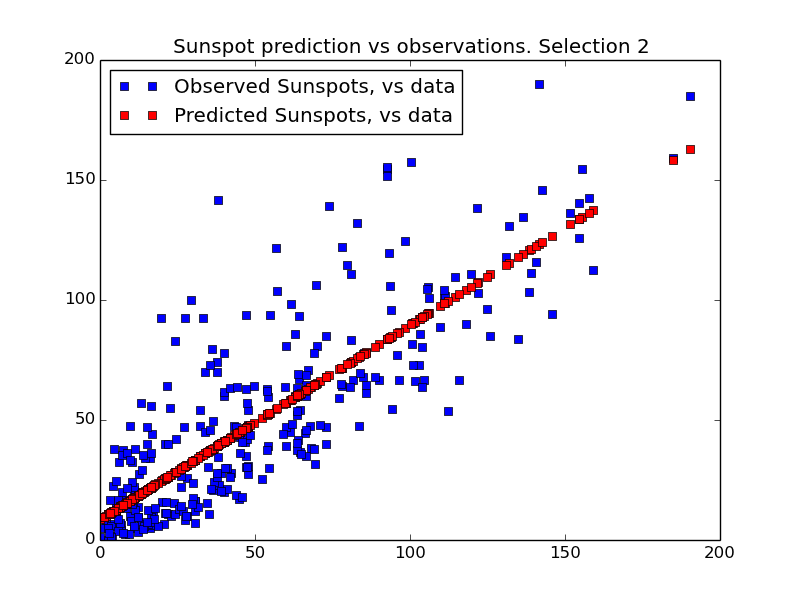
\includegraphics[width=0.5\textwidth]{src/img/predictions_over_obs.png}
%%     \caption{Showing predictions and actual observations as a function of data from selection 2. We clearly see the linearity of the model, but also that the observations do in fact center around a linear line.}
%%     \label{fig:pred_obs}
%% \end{figure}

%% \begin{figure}[h]
%%     \centering
%%     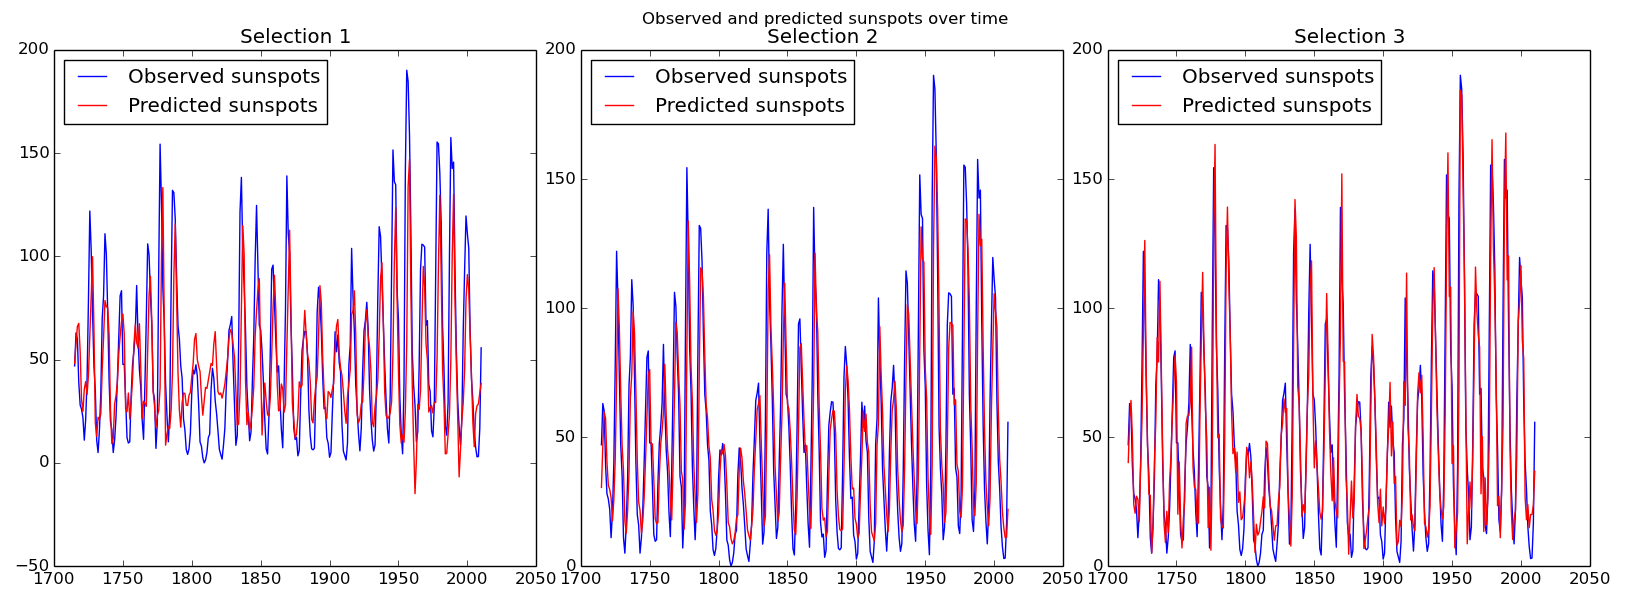
\includegraphics[width=\textwidth]{src/img/obs_over_time}
%%     \caption{Showing how the different selections fit with acutal observations. We see all models account for the recurring ups and downs, but only selection 3 matches all hills and valleys well.}
%%     \label{fig:obs_time}
%% \end{figure}

%% \subsection{II.2.2 Maximum a posteriori solution}

%% Done, see \texttt{src/II.2.2.py}.\\

%% The plots are:\\

%% 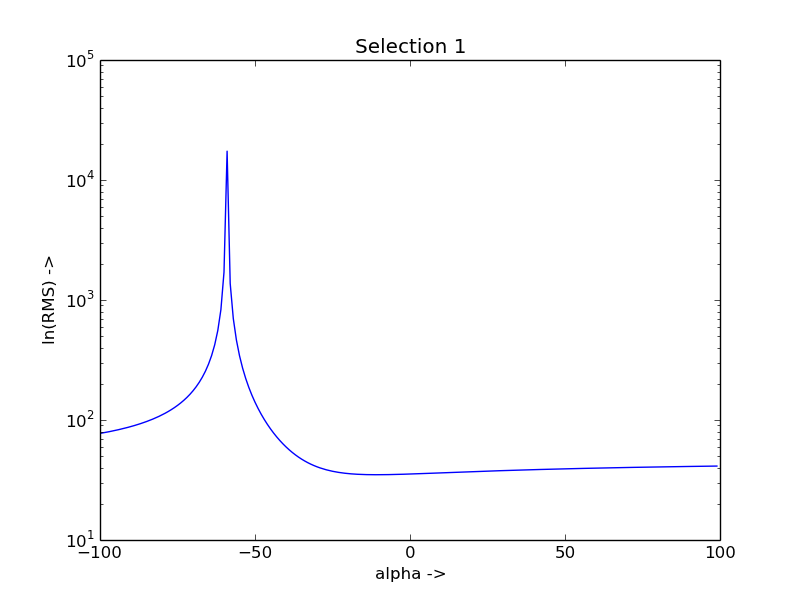
\includegraphics[keepaspectratio=true, width=350pt]{src/img/sel1.png}

%% 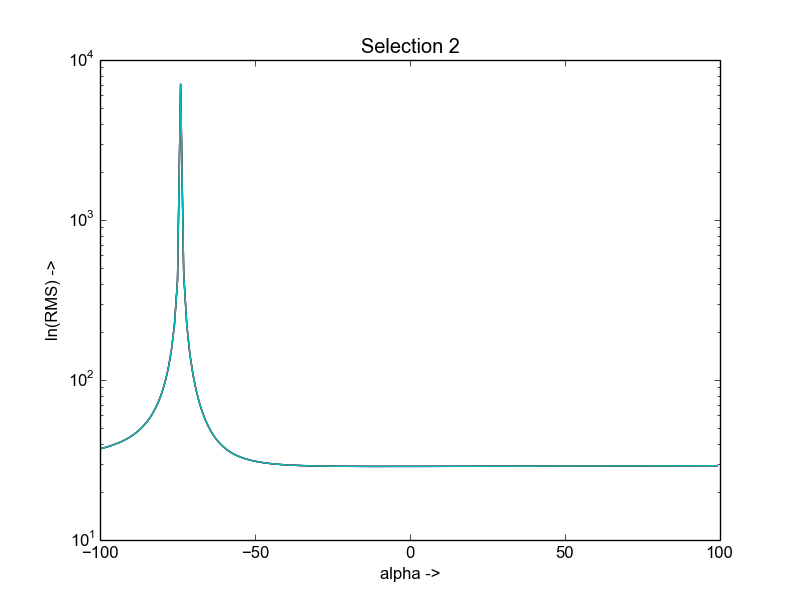
\includegraphics[keepaspectratio=true, width=350pt]{src/img/sel2.png}

%% 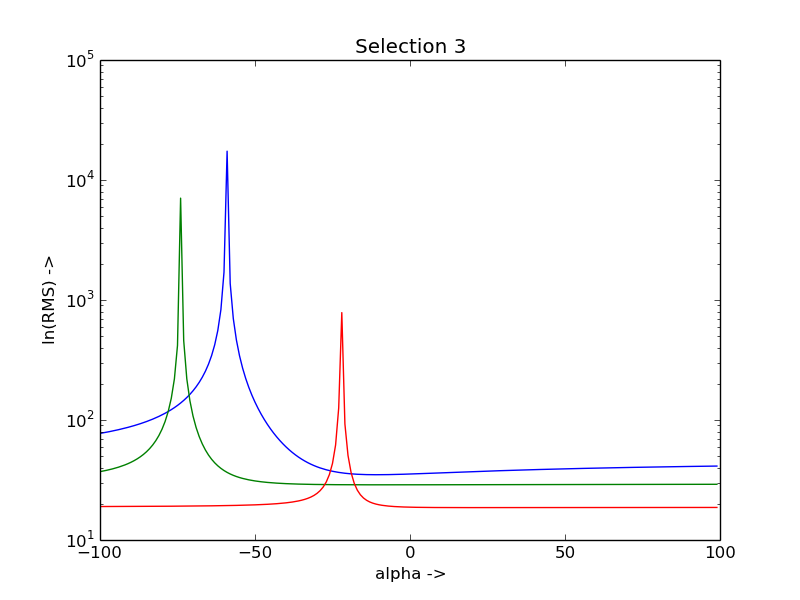
\includegraphics[keepaspectratio=true, width=350pt]{src/img/sel3.png}

%% and combined, along with the RMS of the ML results:\\

%% 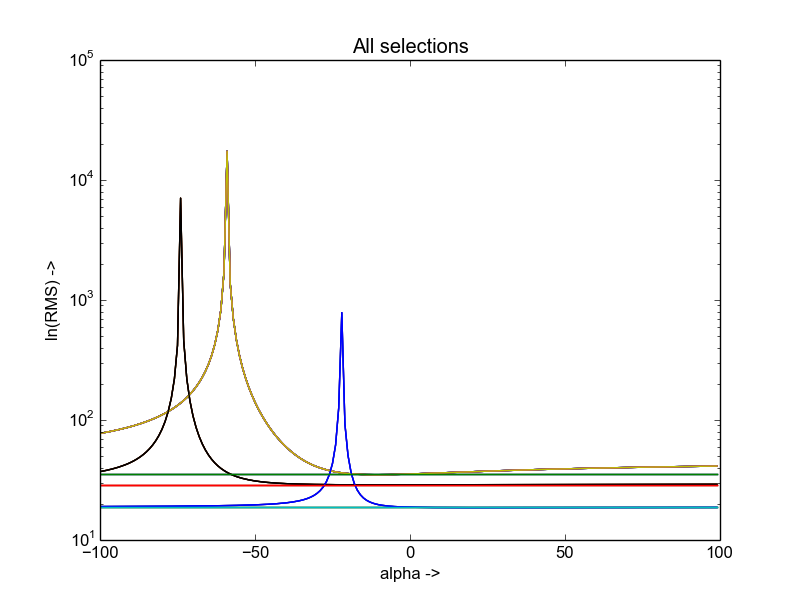
\includegraphics[keepaspectratio=true, width=350pt]{src/img/selall.png}

%% It seems clear that selection 3 provides the best prediction, and selection 1 the worst. The ML solution scores slightly worse for a narrow range of alpha (-11 for Selection 1, -8 for Selection 2 and 22 for Selection 3), but much better for most choices of alpha.


%% \subsection{II.2.3 Weighted sum-of-squares (based on CB Ex. 3.3)}

%% $E_D(\mathbf{w})=\frac{1}{2}\sum_{n=1}^Nr_n\{t_n-\mathbf{w}^T\mathbf{\phi}(\mathbf{x}_n)\}^2$\\

%% To find the minimum we solve $\frac{\delta}{\delta w_i}E_D=0$ for all $i$:\\

%% $\frac{\delta}{\delta w_i}E_D=\sum_{n=1}^Nr_n(t_n-\mathbf{w}^T\mathbf{\phi}(\mathbf{x}_n))\cdot(-\phi_i(\mathbf{x}_n))=0$ for all $i$\\

%% Since $\mathbf{\phi}(\mathbf{x})^T=(\mathbf{\phi}_0(\mathbf{x}),\mathbf{\phi}_1(\mathbf{x}),\dots,\mathbf{\phi}_{n-1}(\mathbf{x}))$, we get\\

%% $\sum_{n=1}^Nr_n\mathbf{w}^T\mathbf{\phi}(\mathbf{x}_n)\mathbf{\phi}(\mathbf{x}_n)^T-\sum_{n=1}^Nr_nt_n\mathbf{\phi}(\mathbf{x}_n)^T=0$\\

%% or\\

%% $0=\mathbf{w}^T\sum_{n=1}^Nr_n\mathbf{\phi}(\mathbf{x}_n)\mathbf{\phi}(\mathbf{x}_n)^T-\sum_{n=1}^N(r_nt_n\mathbf{\phi}(\mathbf{x}_n)^T)$ (*)\\

%% Setting $\Phi=\left(\begin{matrix}\mathbf{\phi}_0(\mathbf{x}_1) & \mathbf{\phi}_1(\mathbf{x}_1) & \dots & \mathbf{\phi}_{M-1}(\mathbf{x}_1) \\
%% \vdots & & & \vdots \\
%% \mathbf{\phi}_0(\mathbf{x}_N) & \mathbf{\phi}_1(\mathbf{x}_N) & \dots & \mathbf{\phi}_{M-1}(\mathbf{x}_N)\end{matrix}\right)$ we rewrite (*) as\\

%% $0=\mathbf{w}^T(\mathbf{\Phi}^T\mathbf{r}\mathbf{\Phi})-\mathbf{r}\mathbf{t}^T\mathbf{\Phi}$\\

%% $\Rightarrow\mathbf{w}^T(\mathbf{\Phi}^T\mathbf{r}\mathbf{\Phi})=\mathbf{r}\mathbf{t}^T\mathbf{\Phi}$\\

%% $\Rightarrow(\mathbf{\Phi}^T\mathbf{r}\mathbf{\Phi})^T\mathbf{w}=(\mathbf{\Phi}^T\mathbf{r}\mathbf{\Phi})\mathbf{w}=\mathbf{\Phi}^T\mathbf{r}\mathbf{t}$\\

%% $\Rightarrow\mathbf{w}^*=(\mathbf{\Phi}^T\mathbf{r}\mathbf{\Phi})^{-1}\mathbf{\Phi}^T\mathbf{r}\mathbf{t}$\\

%% \subsubsection{Data dependent noise variance}

%% If a data point is far from the expected value, the weighting can be used to give that point less importance when minimizing the error.

%% \subsubsection{Replicated data points}

%% Replicated data points will usually hold undue importance, but the weights can be chosen lower for the replicated points to counter this.

%% \newpage

%% Since $\mathbf{\phi}(\mathbf{x})^T=(\mathbf{\phi}_0(\mathbf{x}),\mathbf{\phi}_1(\mathbf{x}),\dots,\mathbf{\phi}_{n-1}(\mathbf{x}))$, we get\\

%% $\sum_{n=1}^Nr_nt_n\mathbf{\phi}(\mathbf{x}_n)^T-\sum_{n=1}^Nr_n\mathbf{w}^T\mathbf{\phi}(\mathbf{x}_n)\mathbf{\phi}(\mathbf{x}_n)^T=0$, so\\

%% $\sum_{n=1}^Nr_nt_n\mathbf{\phi}(\mathbf{x}_n)^T-\mathbf{w}^T\sum_{n=1}^Nr_n\mathbf{\phi}(\mathbf{x}_n)\mathbf{\phi}(\mathbf{x}_n)^T=0$\\

%% Setting $\Phi=\left(\begin{matrix}\mathbf{\phi}_0(\mathbf{x}_1) & \mathbf{\phi}_1(\mathbf{x}_1) & \dots & \mathbf{\phi}_{M-1}(\mathbf{x}_1) \\
%% \vdots & & & \vdots \\
%% \mathbf{\phi}_0(\mathbf{x}_N) & \mathbf{\phi}_1(\mathbf{x}_N) & \dots & \mathbf{\phi}_{M-1}(\mathbf{x}_N)\end{matrix}\right)$ we rewrite as\\

%% $((\mathbf{I}\mathbf{r})\mathbf{t})^T\mathbf{\Phi}-\mathbf{w}^T(\mathbf{\Phi}^T\mathbf{r}\mathbf{\Phi})=0$, or\\

%% $\mathbf{w}^T(\mathbf{\Phi}^T\mathbf{r}\mathbf{\Phi})=((\mathbf{I}\mathbf{r})\mathbf{t})^T\mathbf{\Phi}$, so\\

%% $(\mathbf{\Phi}^T\mathbf{r}\mathbf{\Phi})\mathbf{w}=((\mathbf{I}\mathbf{r})\mathbf{t})^T\mathbf{\Phi}$, thus\\

%% $\mathbf{w}^*=(\mathbf{\Phi}^T\mathbf{r}\mathbf{\Phi})^{-1}((\mathbf{I}\mathbf{r})\mathbf{t})^T\mathbf{\Phi}$, and\\

%% $\mathbf{w}^*=$

% \includegraphics[keepaspectratio=true, width=350pt]{src/img/II_2_3-1.jpg}

% \includegraphics[keepaspectratio=true, width=350pt]{src/img/II_2_3-2.jpg}






\end{document}
